\section{Data processing}

The main objectives of data processing are to enable faster and better decisions by supporting a range of use cases:
\begin{itemize}
    \item \textit{Low latency queries on historical data}: allow for interactive queries on historical data, enabling users to make decisions quickly based on past information.
    \item \textit{Low latency queries on live data}: supports real-time data processing, allowing decisions to be made on live, streaming data as it flows into the system.
    \item \textit{Sophisticated data processing}: enables the execution of more complex, advanced algorithms, which can result in deeper insights and better decision-making.
\end{itemize}
\noindent The goal is to provide comprehensive support for batch, streaming, and interactive computations, and to make it easy to combine these types of processing in a single workflow. 
This approach simplifies the development of sophisticated algorithms that can handle various forms of data in a flexible manner.

\subsection{Hadoop}
Hadoop is responsible for storing data across a cluster, with data files split into blocks and distributed across the nodes.
These blocks are replicated multiple times for redundancy, providing reliable storage for large amounts of data. 
Hadoop Distributed File System is optimized for streaming reads of large files, typically 100MB or more, and is designed for a write-once-read-many access model.
\begin{figure}[H]
    \centering
    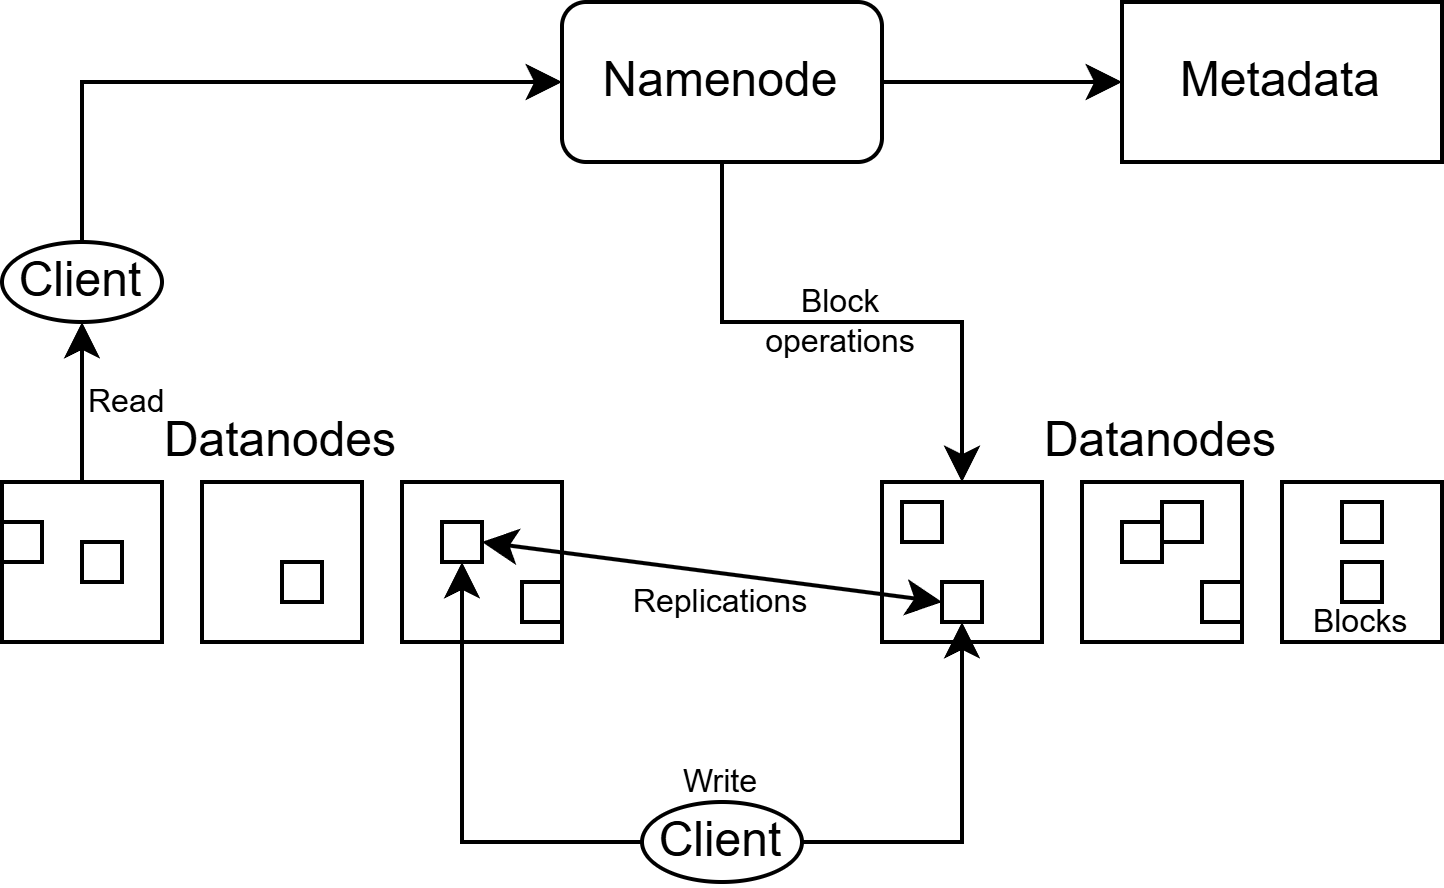
\includegraphics[width=0.75\linewidth]{images/hadoop.png}
    \caption{Hadoop architecture}
\end{figure}
The key components and features are: 
\begin{itemize}
    \item \textit{NameNode}: manages the file system namespace, keeps track of where each file's blocks are stored, and handles cluster configuration and replication.
        It maintains metadata such as the list of files, blocks, and DataNodes.
    \item \textit{DataNode}: stores the actual data and metadata of blocks, serves data to clients, and periodically reports block information to the NameNode. 
        It also facilitates data pipelining, where blocks are forwarded to other DataNodes.
    \item \textit{Block replication}: blocks are replicated across multiple DataNodes to ensure data availability. 
        A typical strategy places one replica on the local node, another on a remote rack, and a third on the same remote rack.
    \item \textit{Fault tolerance}: the system uses heartbeats to detect DataNode failures, and the NameNode will replicate blocks to other DataNodes if a failure is detected. 
        Clients can access data directly from the nearest replica, ensuring fast data retrieval.
    \item \textit{Metadata and data consistency}: the NameNode stores metadata in memory, and DataNodes use checksums to validate data integrity. 
        In case of NameNode failure, transaction logs are stored in multiple locations to prevent data loss.
    \item \textit{Cluster maintenance}: Hadoop includes a Rebalancer to balance disk usage across DataNodes and a Secondary NameNode to merge transaction logs and maintain the file system's integrity.
    \item \textit{Authentication and security}: Hadoop supports two authentication mechanisms: simple OS-based authentication and more secure Kerberos authentication. 
        File and directory permissions are similar to POSIX standards, with access control lists allowing for fine-grained permissions.
\end{itemize}

\subsection{Spark}
Apache Spark is an open-source project that has gained tremendous popularity since its first release in February 2013. 
It quickly became a go-to solution for big data processing due to its ease of use and speed. 
Spark was originally created at the AMPLab at the University of California, Berkeley, and has since become a core part of the modern data analytics ecosystem.
\begin{figure}[H]
    \centering
    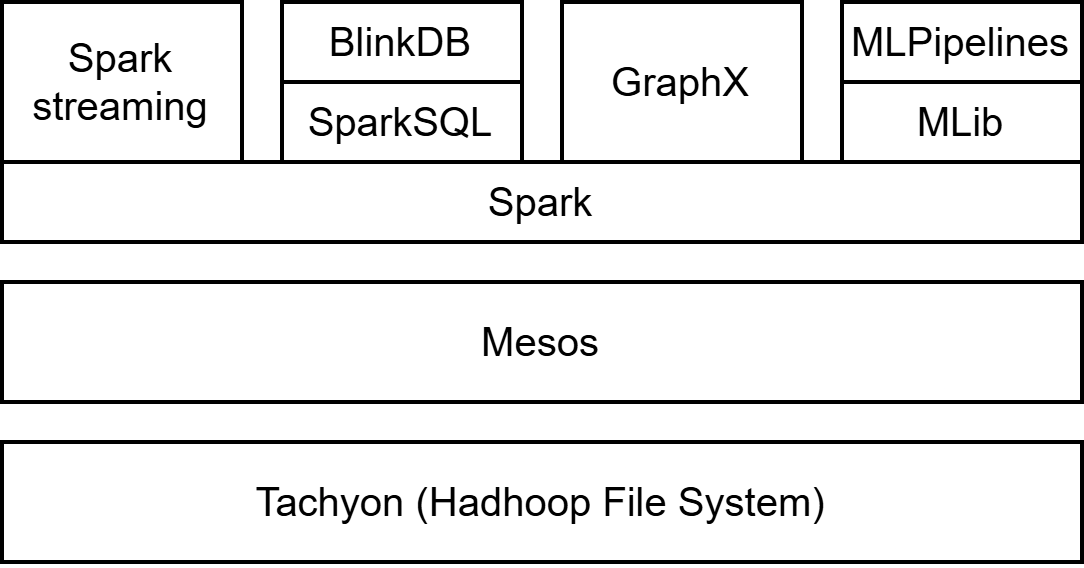
\includegraphics[width=0.75\linewidth]{images/spark.png}
    \caption{Spark architecture}
\end{figure}
Spark is a powerful, fault-tolerant, in-memory storage system using Resilient Distributed Datasets.
It offers fast performance and is easy to use, with 5-10x less code than Hadoop. 
It supports a variety of programming models, including interactive and iterative applications, and is scalable across clusters.
The key features are: 
\begin{itemize}
    \item \textit{Fault-tolerant}: Spark handles failures efficiently by tracking the lineage of Resilient Distributed Datasets.
    \item \textit{Unified programming models}: Spark supports SQL, graph processing, and Machine Learning, all within the same framework.
    \item \textit{Streaming}: Spark streaming allows large-scale, fault-tolerant streaming computations, integrating batch, interactive, and streaming processes.
    \item \textit{SparkSQL}: offers full support for HiveQL and UDFs, providing SQL-based querying for Spark data.
    \item \textit{Performance}: Spark is faster than Hadoop, especially when data is stored in memory, and supports large-scale data storage systems.
\end{itemize}
Resilient Distributed Datasets are the core data structure in Spark, representing a distributed collection of data that is fault-tolerant and supports parallel operations. 
Resilient Distributed Datasets allow for operations like map, filter, and join, which are lazily evaluated (executed only when an action is called): 
\begin{itemize}
    \item \textit{Transformations}: operations like map and filter create new Resilient Distributed Datasets but are not executed immediately.
    \item \textit{Actions}: operations like count and collect trigger execution and return results.
\end{itemize}
Data frames are immutable collections of data with named columns built on top of Resilient Distributed Datasets. 
They offer a user-friendly API, uniform functionality across languages, and performance optimizations.

\subsubsection{Parquet}
Apache Parquet is a columnar storage format optimized for high compression and scan efficiency, commonly used in the Hadoop and Spark ecosystems. 
It is ideal for storing nested data and is supported by most data processing frameworks. The columnar format uses definition and repetition levels to store data, which is highly efficient for analytic workloads.

Optimized for analytical queries by allowing fast scans of specific columns.
Supports high compression ratios, making it ideal for storing large datasets efficiently.
Parquet works across multiple languages and data processing frameworks.